% !TEX root = ../main.tex
\section{Experiments}


\begin{figure}[ht]
    \begin{subfigure}{\linewidth}
    \centering
    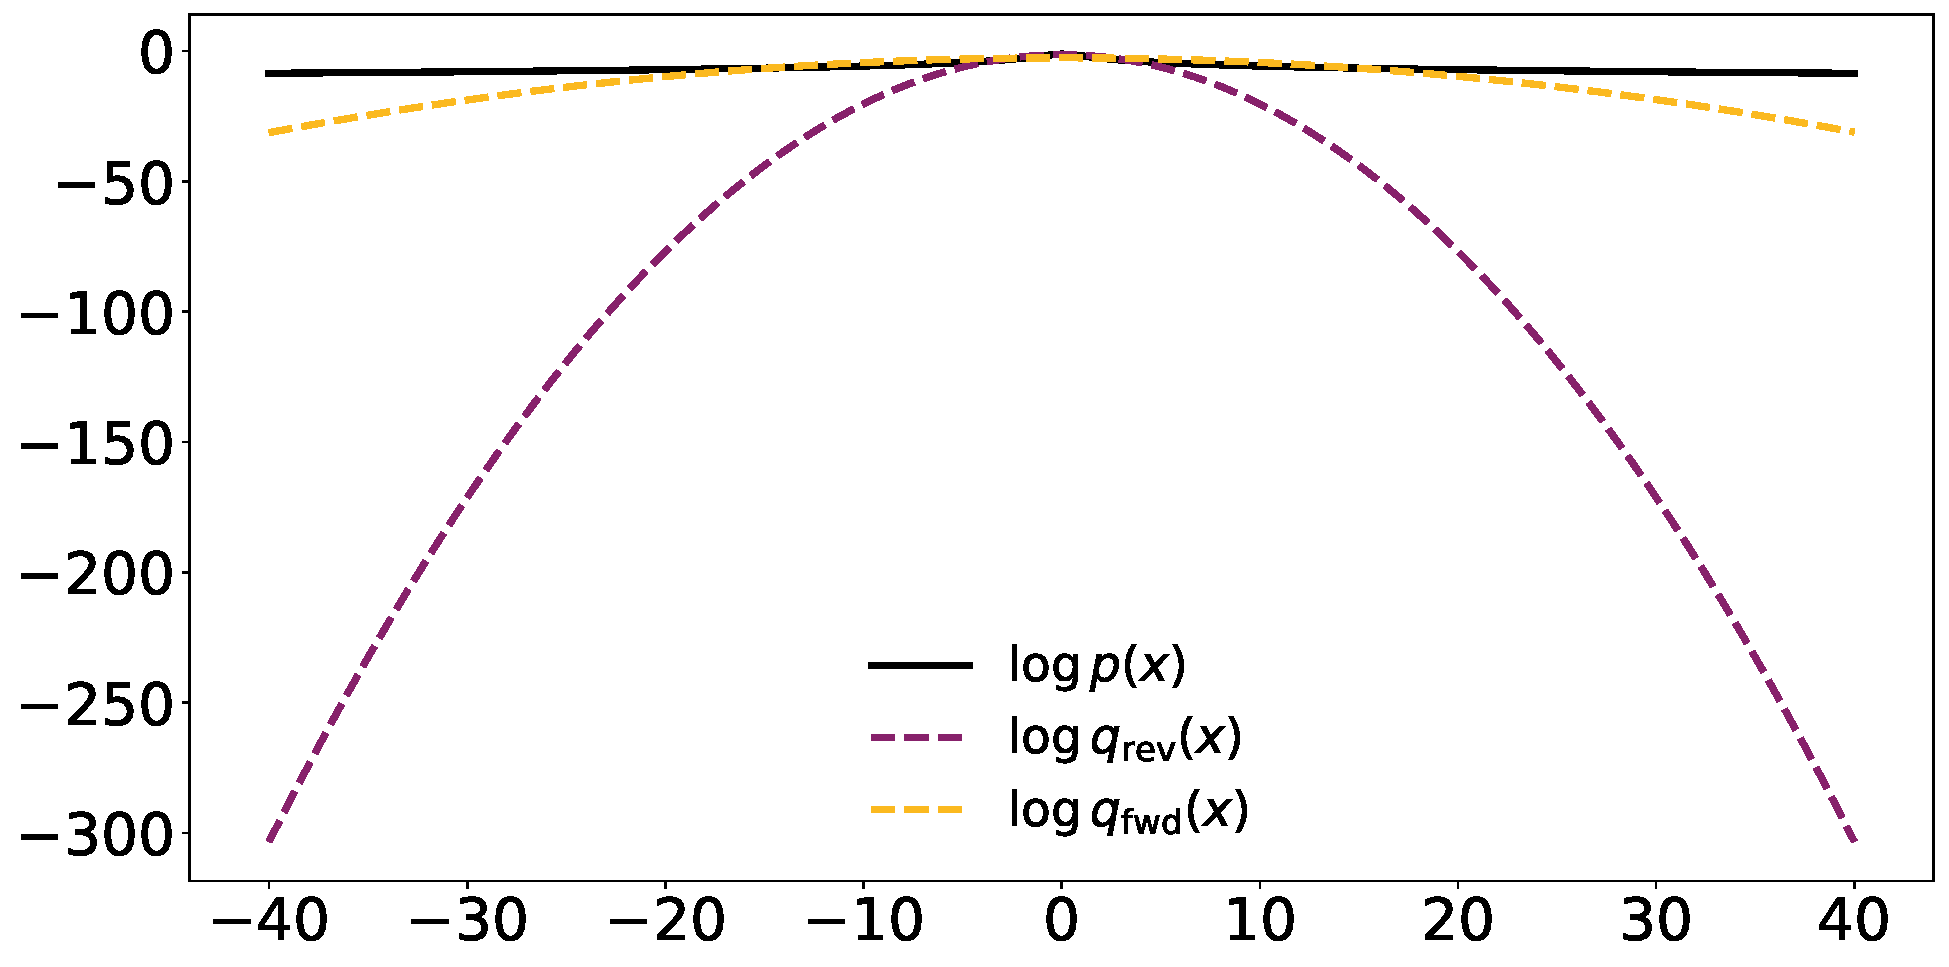
\includegraphics[width=0.8\linewidth]{fig/cauchy_logq.pdf}
    \caption{Log density}
    \label{fig:cauchy_lp}
    \end{subfigure}\\[1ex]
    \begin{subfigure}{\linewidth}
    \centering
    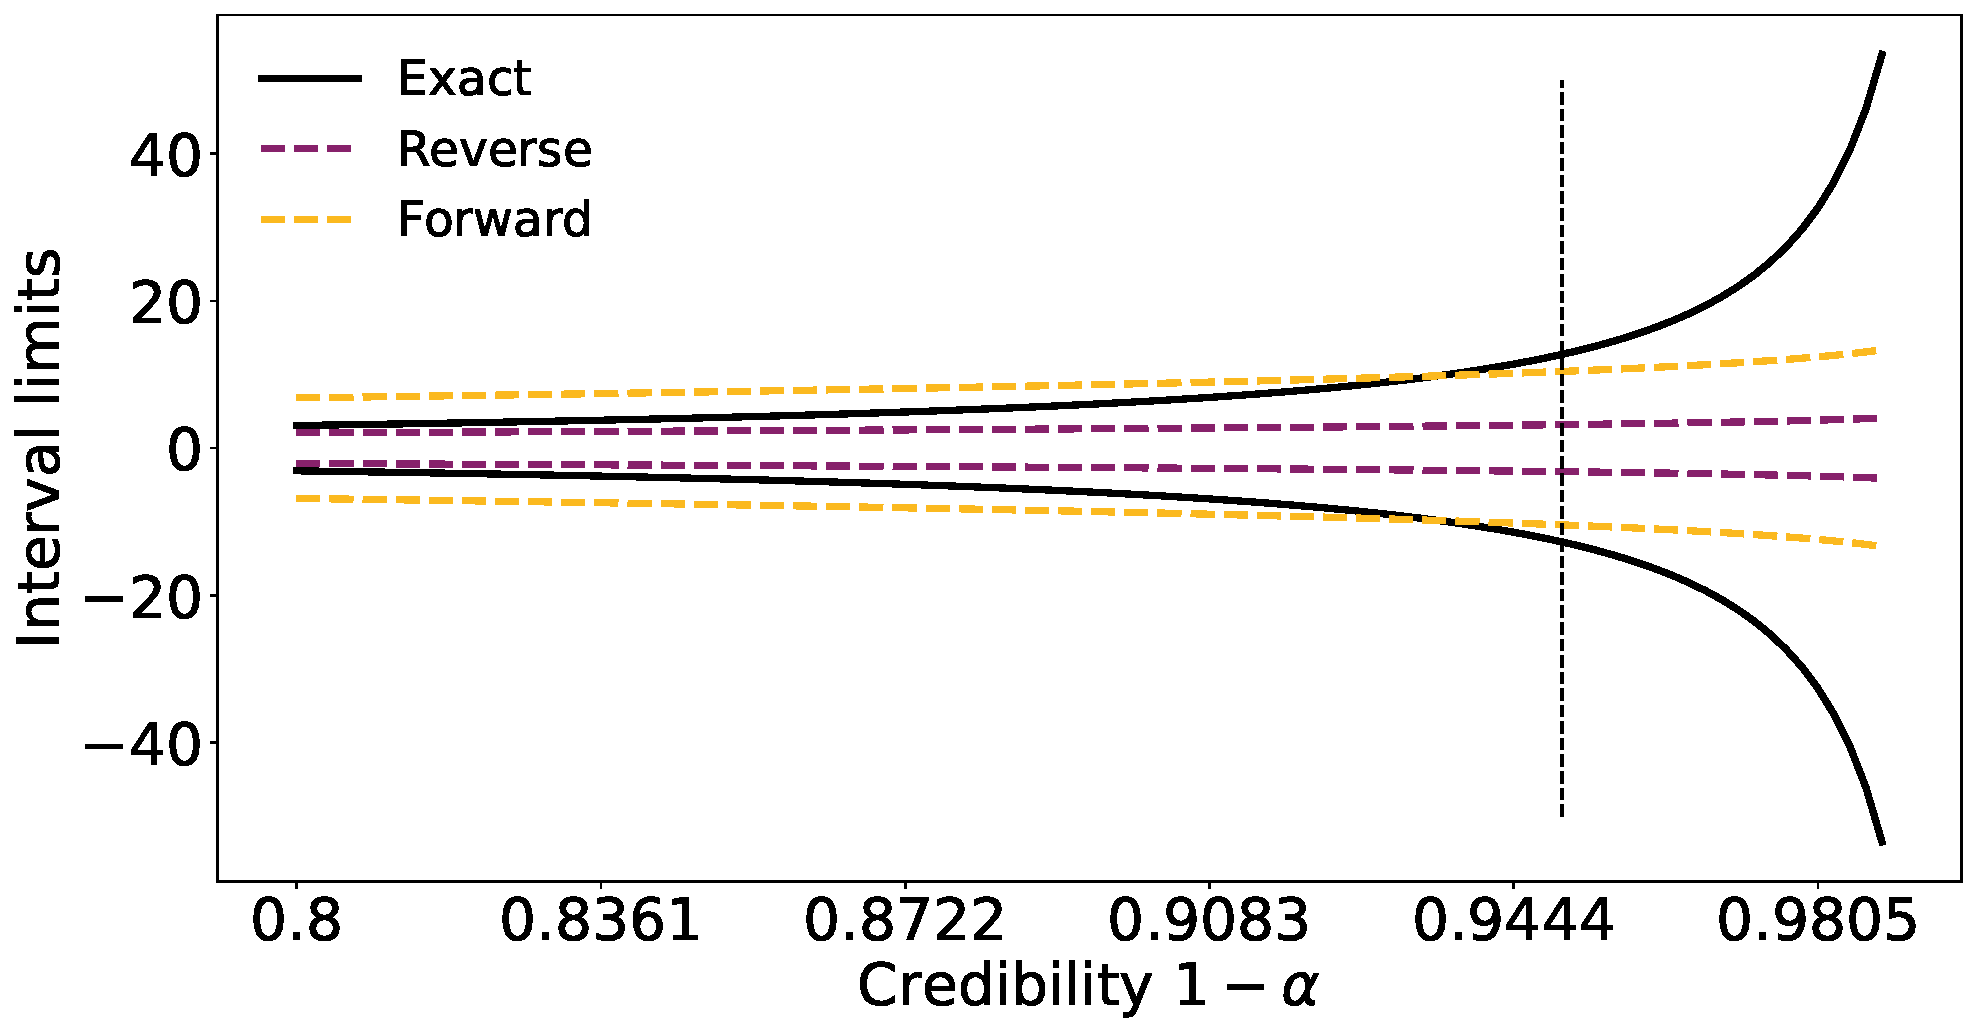
\includegraphics[width=0.8\linewidth]{fig/cauchy_cilims.pdf}
    \caption{CI limits}
    \label{fig:cauchy_lims}
    \end{subfigure}\\[1ex]
    \begin{subfigure}{\linewidth}
    \centering
    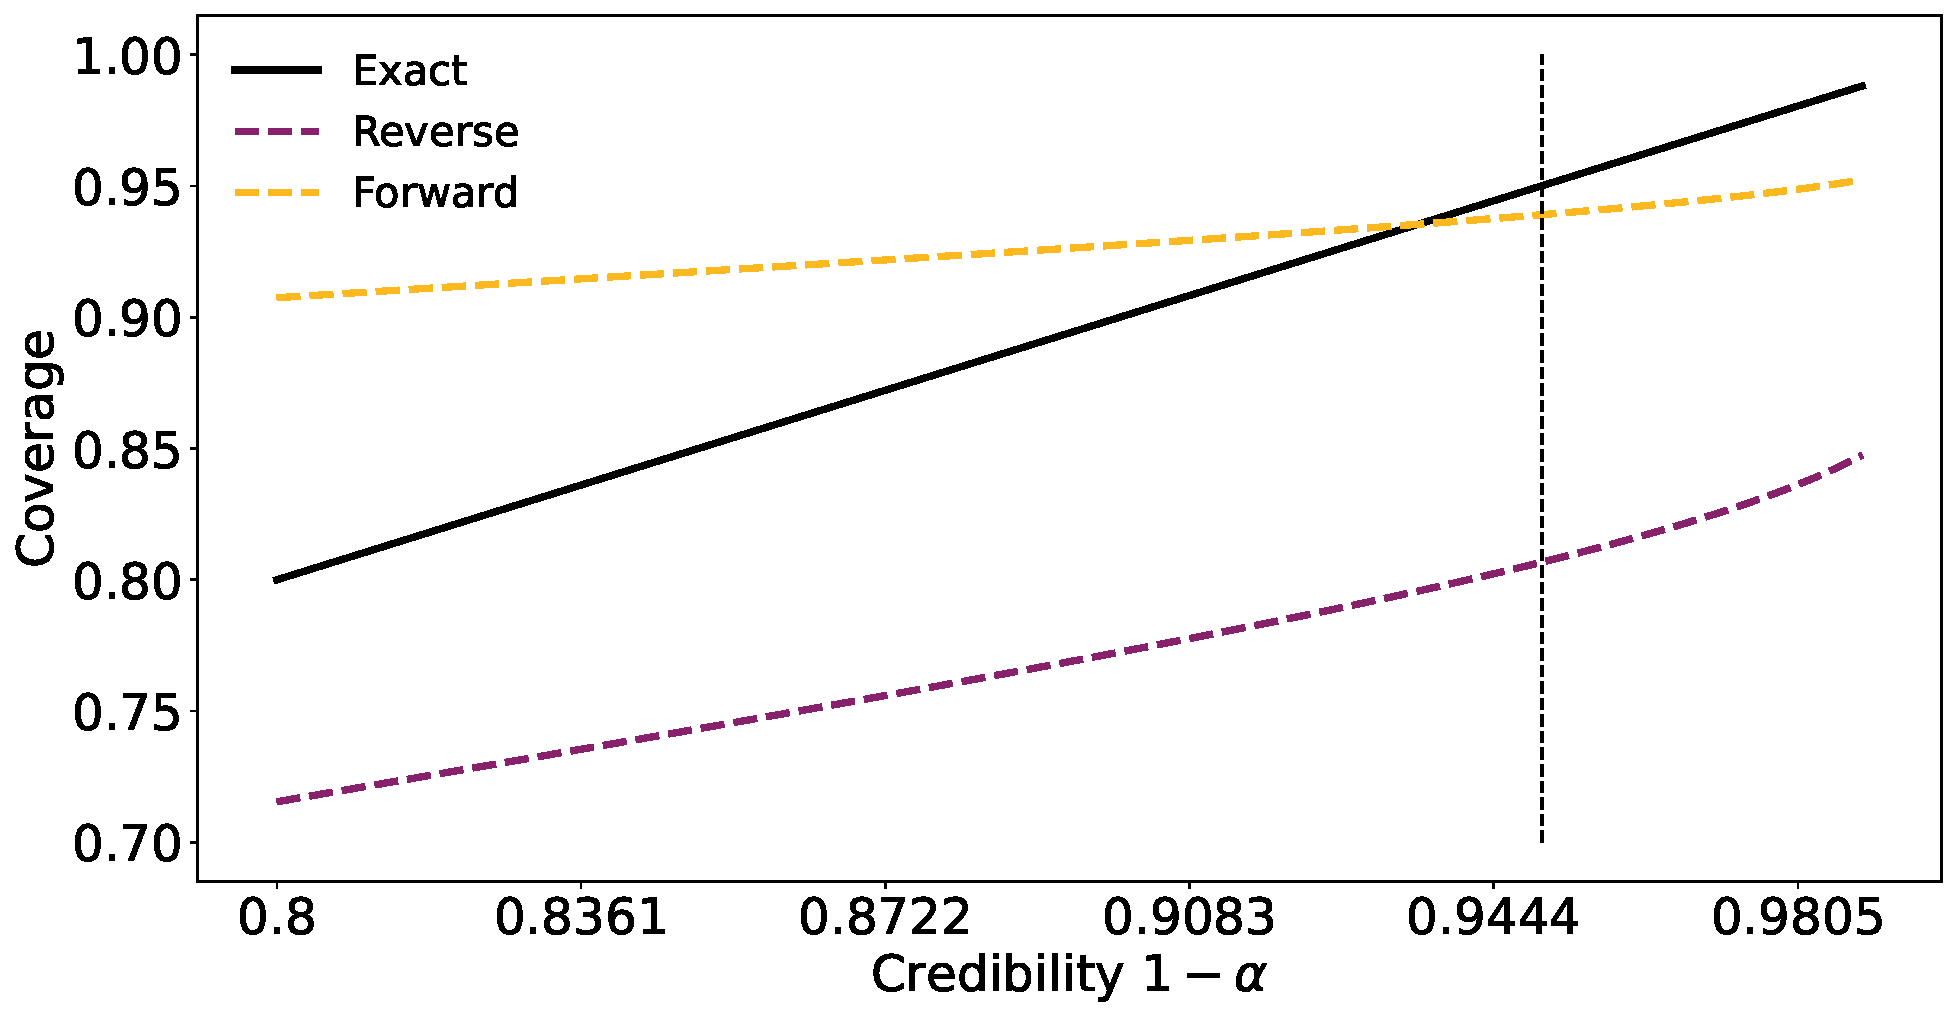
\includegraphics[width=0.8\linewidth]{fig/cauchy_cicoverage.pdf}
    \caption{CI coverage}
    \label{fig:cauchy_coverage}
    \end{subfigure}
    \caption{Results on the Cauchy distribution.}
    \label{fig:cauchy}
    \end{figure}